% Diagrama teórico de tren de pulsos en tiempo y frecuencia (Consigna pág. 7)
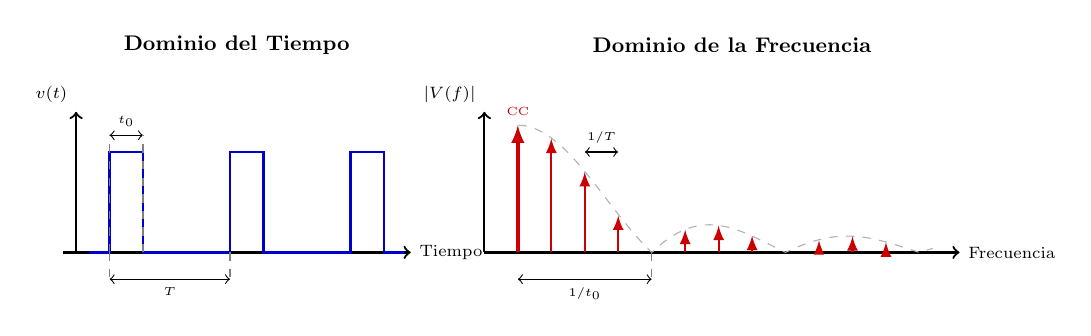
\begin{tikzpicture}[scale=0.85, transform shape]
    % Dominio del tiempo
    \begin{scope}[shift={(0,0)}]
        \node at (2.4, 3.1) [font=\small\bfseries] {Dominio del Tiempo};
        \draw[->, thick] (-0.2,0) -- (5.0,0) node[right, font=\scriptsize] {Tiempo};
        \draw[->, thick] (0,0) -- (0,2.1) node[above left, font=\scriptsize] {$v(t)$};
        
        % Pulsos rectangulares
        \draw[blue!80!black, thick] (0.2,0) -- (0.5,0) -- (0.5,1.5) -- (1.0,1.5) -- (1.0,0) 
            -- (2.3,0) -- (2.3,1.5) -- (2.8,1.5) -- (2.8,0) 
            -- (4.1,0) -- (4.1,1.5) -- (4.6,1.5) -- (4.6,0) -- (4.9,0);

        % Cotas to y T
        \draw[<->, font=\tiny] (0.5,1.75) -- (1.0,1.75) node[midway, above] {$t_0$};
        \draw[dashed, gray] (0.5,0) -- (0.5,1.75);
        \draw[dashed, gray] (1.0,0) -- (1.0,1.75);

        \draw[<->, font=\tiny] (0.5,-0.4) -- (2.3,-0.4) node[midway, below] {$T$};
        \draw[dashed, gray] (0.5,0) -- (0.5,-0.4);
        \draw[dashed, gray] (2.3,0) -- (2.3,-0.4);
    \end{scope}

    % Dominio de la frecuencia (Espectro con envolvente sinc positiva en DSO)
    \begin{scope}[shift={(6.6,0)}]
        \node at (3.2, 3.1) [font=\small\bfseries] {Dominio de la Frecuencia};
        \draw[->, thick] (-0.5,0) -- (6.6,0) node[right, font=\scriptsize] {Frecuencia};
        \draw[->, thick] (-0.5,0) -- (-0.5,2.1) node[above left, font=\scriptsize] {$|V(f)|$};

        % Envolvente sinc (módulo en pantalla del osciloscopio)
        \draw[gray!60, dashed, domain=0.01:6.2, samples=150, smooth] 
            plot (\x, {1.9*abs(sin(deg(\x*1.5708))/(\x*1.5708))});

        % Rayas espectrales espaciadas por 1/T
        \draw[red!80!black, very thick, -latex] (0,0) -- (0,1.9) node[above, font=\tiny] {CC};
        \draw[red!80!black, thick, -latex] (0.5,0) -- (0.5,1.7);
        \draw[red!80!black, thick, -latex] (1.0,0) -- (1.0,1.2);
        \draw[red!80!black, thick, -latex] (1.5,0) -- (1.5,0.55);
        % En 2.0 hay un cero (4 kHz)
        \draw[red!80!black, thick, -latex] (2.5,0) -- (2.5,0.34);
        \draw[red!80!black, thick, -latex] (3.0,0) -- (3.0,0.40);
        \draw[red!80!black, thick, -latex] (3.5,0) -- (3.5,0.25);
        % En 4.0 hay otro cero (8 kHz)
        \draw[red!80!black, thick, -latex] (4.5,0) -- (4.5,0.18);
        \draw[red!80!black, thick, -latex] (5.0,0) -- (5.0,0.24);
        \draw[red!80!black, thick, -latex] (5.5,0) -- (5.5,0.15);

        % Cotas 1/T y 1/to
        \draw[<->, font=\tiny] (1.0,1.5) -- (1.5,1.5) node[midway, above] {$1/T$};
        \draw[<->, font=\tiny] (0,-0.4) -- (2.0,-0.4) node[midway, below] {$1/t_0$};
        \draw[dashed, gray] (2.0,0) -- (2.0,-0.4);
    \end{scope}
\end{tikzpicture}
